\documentclass[1p]{elsarticle_modified}
%\bibliographystyle{elsarticle-num}

%\usepackage[colorlinks]{hyperref}
%\usepackage{abbrmath_seonhwa} %\Abb, \Ascr, \Acal ,\Abf, \Afrak
\usepackage{amsfonts}
\usepackage{amssymb}
\usepackage{amsmath}
\usepackage{amsthm}
\usepackage{scalefnt}
\usepackage{amsbsy}
\usepackage{kotex}
\usepackage{caption}
\usepackage{subfig}
\usepackage{color}
\usepackage{graphicx}
\usepackage{xcolor} %% white, black, red, green, blue, cyan, magenta, yellow
\usepackage{float}
\usepackage{setspace}
\usepackage{hyperref}

\usepackage{tikz}
\usetikzlibrary{arrows}

\usepackage{multirow}
\usepackage{array} % fixed length table
\usepackage{hhline}

%%%%%%%%%%%%%%%%%%%%%
\makeatletter
\renewcommand*\env@matrix[1][\arraystretch]{%
	\edef\arraystretch{#1}%
	\hskip -\arraycolsep
	\let\@ifnextchar\new@ifnextchar
	\array{*\c@MaxMatrixCols c}}
\makeatother %https://tex.stackexchange.com/questions/14071/how-can-i-increase-the-line-spacing-in-a-matrix
%%%%%%%%%%%%%%%

\usepackage[normalem]{ulem}

\newcommand{\msout}[1]{\ifmmode\text{\sout{\ensuremath{#1}}}\else\sout{#1}\fi}
%SOURCE: \msout is \stkout macro in https://tex.stackexchange.com/questions/20609/strikeout-in-math-mode

\newcommand{\cancel}[1]{
	\ifmmode
	{\color{red}\msout{#1}}
	\else
	{\color{red}\sout{#1}}
	\fi
}

\newcommand{\add}[1]{
	{\color{blue}\uwave{#1}}
}

\newcommand{\replace}[2]{
	\ifmmode
	{\color{red}\msout{#1}}{\color{blue}\uwave{#2}}
	\else
	{\color{red}\sout{#1}}{\color{blue}\uwave{#2}}
	\fi
}

\newcommand{\Sol}{\mathcal{S}} %segment
\newcommand{\D}{D} %diagram
\newcommand{\A}{\mathcal{A}} %arc


%%%%%%%%%%%%%%%%%%%%%%%%%%%%%5 test

\def\sl{\operatorname{\textup{SL}}(2,\Cbb)}
\def\psl{\operatorname{\textup{PSL}}(2,\Cbb)}
\def\quan{\mkern 1mu \triangleright \mkern 1mu}

\theoremstyle{definition}
\newtheorem{thm}{Theorem}[section]
\newtheorem{prop}[thm]{Proposition}
\newtheorem{lem}[thm]{Lemma}
\newtheorem{ques}[thm]{Question}
\newtheorem{cor}[thm]{Corollary}
\newtheorem{defn}[thm]{Definition}
\newtheorem{exam}[thm]{Example}
\newtheorem{rmk}[thm]{Remark}
\newtheorem{alg}[thm]{Algorithm}

\newcommand{\I}{\sqrt{-1}}
\begin{document}

%\begin{frontmatter}
%
%\title{Boundary parabolic representations of knots up to 8 crossings}
%
%%% Group authors per affiliation:
%\author{Yunhi Cho} 
%\address{Department of Mathematics, University of Seoul, Seoul, Korea}
%\ead{yhcho@uos.ac.kr}
%
%
%\author{Seonhwa Kim} %\fnref{s_kim}}
%\address{Center for Geometry and Physics, Institute for Basic Science, Pohang, 37673, Korea}
%\ead{ryeona17@ibs.re.kr}
%
%\author{Hyuk Kim}
%\address{Department of Mathematical Sciences, Seoul National University, Seoul 08826, Korea}
%\ead{hyukkim@snu.ac.kr}
%
%\author{Seokbeom Yoon}
%\address{Department of Mathematical Sciences, Seoul National University, Seoul, 08826,  Korea}
%\ead{sbyoon15@snu.ac.kr}
%
%\begin{abstract}
%We find all boundary parabolic representation of knots up to 8 crossings.
%
%\end{abstract}
%\begin{keyword}
%    \MSC[2010] 57M25 
%\end{keyword}
%
%\end{frontmatter}

%\linenumbers
%\tableofcontents
%
\newcommand\colored[1]{\textcolor{white}{\rule[-0.35ex]{0.8em}{1.4ex}}\kern-0.8em\color{red} #1}%
%\newcommand\colored[1]{\textcolor{white}{ #1}\kern-2.17ex	\textcolor{white}{ #1}\kern-1.81ex	\textcolor{white}{ #1}\kern-2.15ex\color{red}#1	}

{\Large $\underline{12a_{1140}~(K12a_{1140})}$}

\setlength{\tabcolsep}{10pt}
\renewcommand{\arraystretch}{1.6}
\vspace{1cm}\begin{tabular}{m{100pt}>{\centering\arraybackslash}m{274pt}}
\multirow{5}{120pt}{
	\centering
	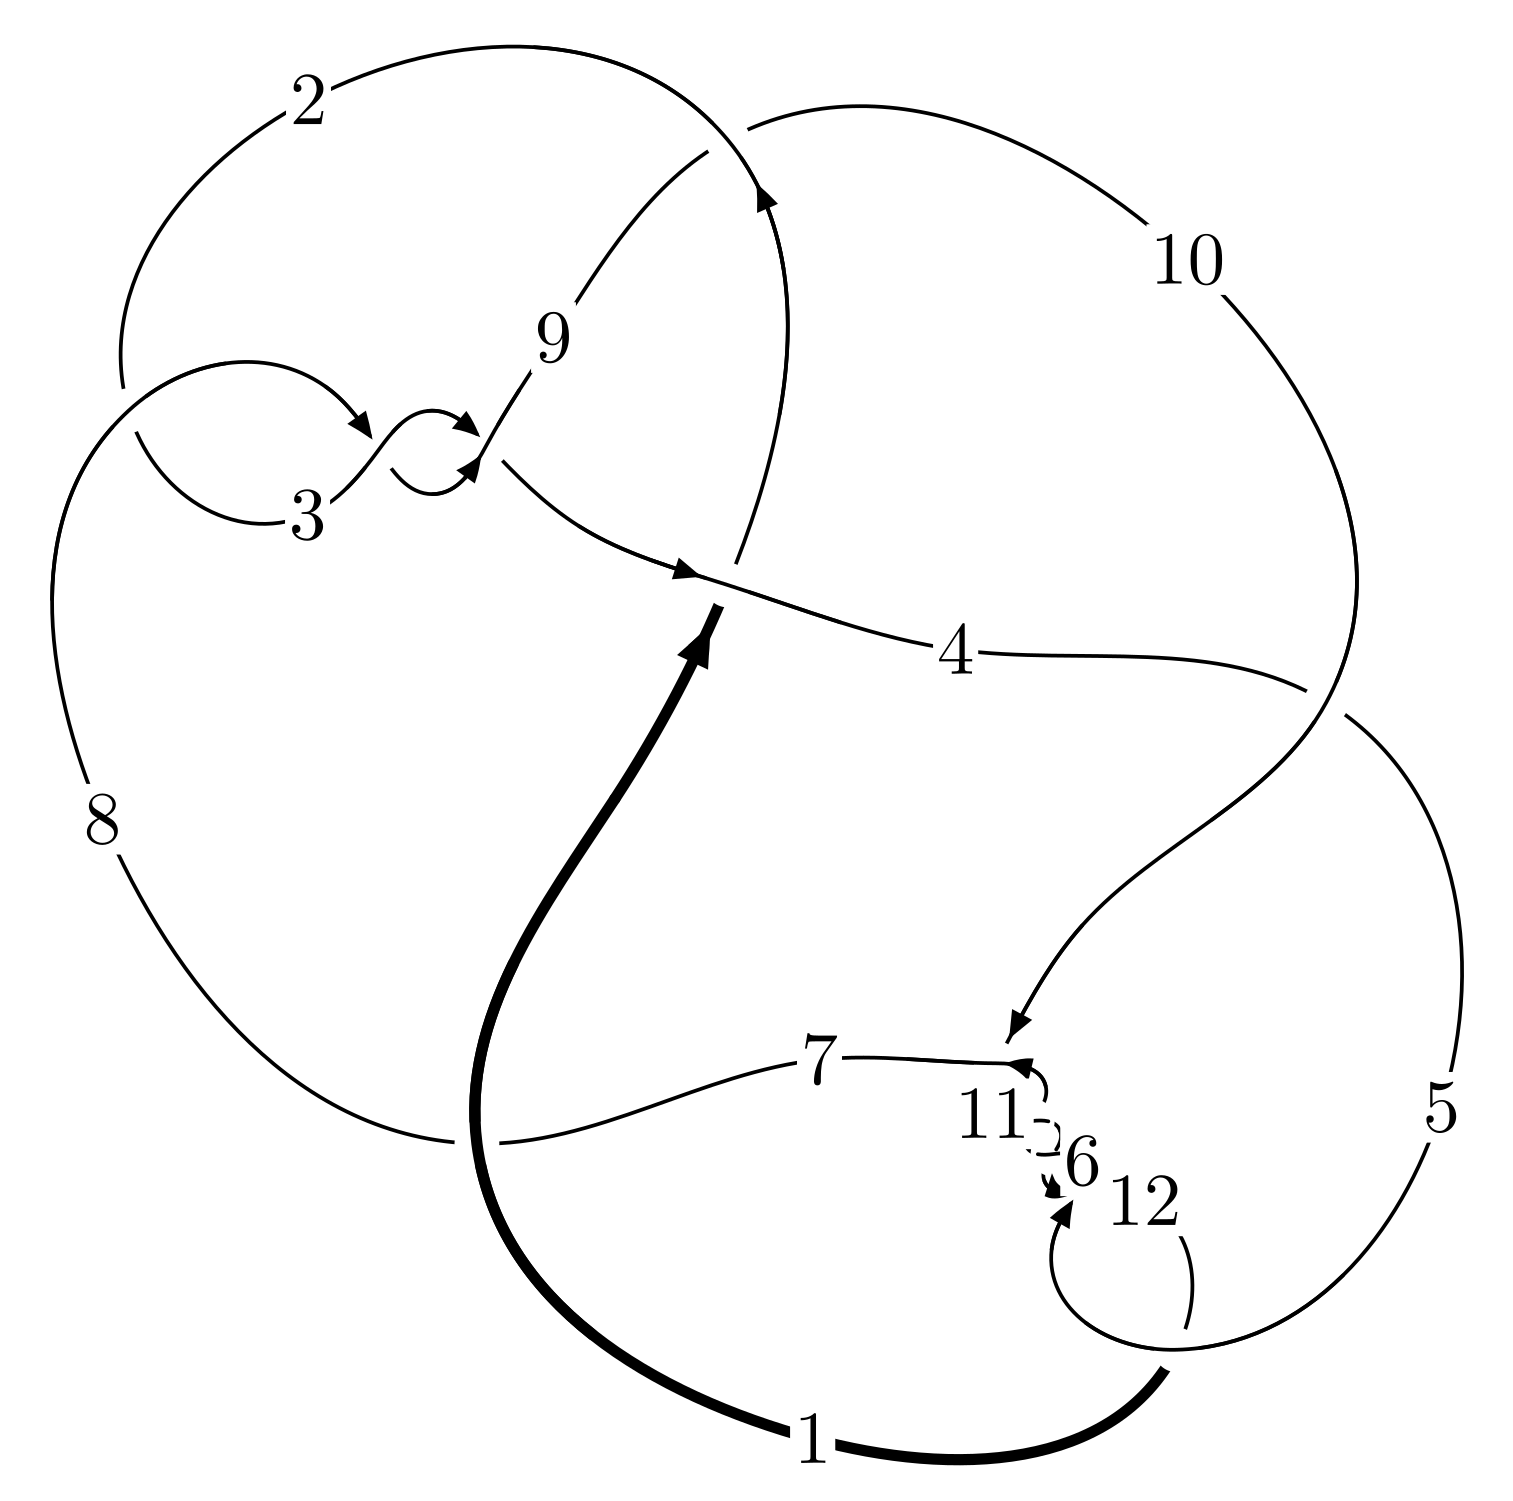
\includegraphics[width=112pt]{../../../GIT/diagram.site/Diagrams/png/1941_12a_1140.png}\\
\ \ \ A knot diagram\footnotemark}&
\allowdisplaybreaks
\textbf{Linearized knot diagam} \\
\cline{2-2}
 &
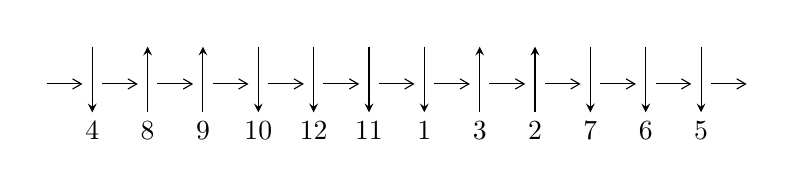
\begin{tikzpicture}[x=20pt, y=17pt]
	% nodes
	\node (C0) at (0, 0) {};
	\node (C1) at (1, 0) {};
	\node (C1U) at (1, +1) {};
	\node (C1D) at (1, -1) {4};

	\node (C2) at (2, 0) {};
	\node (C2U) at (2, +1) {};
	\node (C2D) at (2, -1) {8};

	\node (C3) at (3, 0) {};
	\node (C3U) at (3, +1) {};
	\node (C3D) at (3, -1) {9};

	\node (C4) at (4, 0) {};
	\node (C4U) at (4, +1) {};
	\node (C4D) at (4, -1) {10};

	\node (C5) at (5, 0) {};
	\node (C5U) at (5, +1) {};
	\node (C5D) at (5, -1) {12};

	\node (C6) at (6, 0) {};
	\node (C6U) at (6, +1) {};
	\node (C6D) at (6, -1) {11};

	\node (C7) at (7, 0) {};
	\node (C7U) at (7, +1) {};
	\node (C7D) at (7, -1) {1};

	\node (C8) at (8, 0) {};
	\node (C8U) at (8, +1) {};
	\node (C8D) at (8, -1) {3};

	\node (C9) at (9, 0) {};
	\node (C9U) at (9, +1) {};
	\node (C9D) at (9, -1) {2};

	\node (C10) at (10, 0) {};
	\node (C10U) at (10, +1) {};
	\node (C10D) at (10, -1) {7};

	\node (C11) at (11, 0) {};
	\node (C11U) at (11, +1) {};
	\node (C11D) at (11, -1) {6};

	\node (C12) at (12, 0) {};
	\node (C12U) at (12, +1) {};
	\node (C12D) at (12, -1) {5};
	\node (C13) at (13, 0) {};

	% arrows
	\draw[->,>={angle 60}]
	(C0) edge (C1) (C1) edge (C2) (C2) edge (C3) (C3) edge (C4) (C4) edge (C5) (C5) edge (C6) (C6) edge (C7) (C7) edge (C8) (C8) edge (C9) (C9) edge (C10) (C10) edge (C11) (C11) edge (C12) (C12) edge (C13) ;	\draw[->,>=stealth]
	(C1U) edge (C1D) (C2D) edge (C2U) (C3D) edge (C3U) (C4U) edge (C4D) (C5U) edge (C5D) (C6U) edge (C6D) (C7U) edge (C7D) (C8D) edge (C8U) (C9D) edge (C9U) (C10U) edge (C10D) (C11U) edge (C11D) (C12U) edge (C12D) ;
	\end{tikzpicture} \\
\hhline{~~} \\& 
\textbf{Solving Sequence} \\ \cline{2-2} 
 &
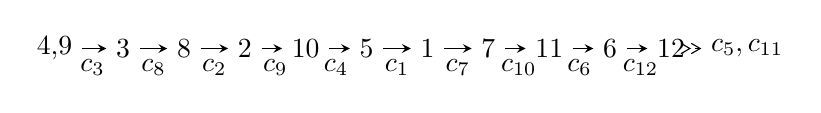
\begin{tikzpicture}[x=22pt, y=7pt]
	% node
	\node (A0) at (-1/8, 0) {4,9};
	\node (A1) at (1, 0) {3};
	\node (A2) at (2, 0) {8};
	\node (A3) at (3, 0) {2};
	\node (A4) at (4, 0) {10};
	\node (A5) at (5, 0) {5};
	\node (A6) at (6, 0) {1};
	\node (A7) at (7, 0) {7};
	\node (A8) at (8, 0) {11};
	\node (A9) at (9, 0) {6};
	\node (A10) at (10, 0) {12};
	\node (C1) at (1/2, -1) {$c_{3}$};
	\node (C2) at (3/2, -1) {$c_{8}$};
	\node (C3) at (5/2, -1) {$c_{2}$};
	\node (C4) at (7/2, -1) {$c_{9}$};
	\node (C5) at (9/2, -1) {$c_{4}$};
	\node (C6) at (11/2, -1) {$c_{1}$};
	\node (C7) at (13/2, -1) {$c_{7}$};
	\node (C8) at (15/2, -1) {$c_{10}$};
	\node (C9) at (17/2, -1) {$c_{6}$};
	\node (C10) at (19/2, -1) {$c_{12}$};
	\node (A11) at (45/4, 0) {$c_{5},c_{11}$};

	% edge
	\draw[->,>=stealth]	
	(A0) edge (A1) (A1) edge (A2) (A2) edge (A3) (A3) edge (A4) (A4) edge (A5) (A5) edge (A6) (A6) edge (A7) (A7) edge (A8) (A8) edge (A9) (A9) edge (A10) ;
	\draw[->>,>={angle 60}]	
	(A10) edge (A11);
\end{tikzpicture} \\ 

\end{tabular} \\

\footnotetext{
The image of knot diagram is generated by the software ``\textbf{Draw programme}" developed by Andrew Bartholomew(\url{http://www.layer8.co.uk/maths/draw/index.htm\#Running-draw}), where we modified some parts for our purpose(\url{https://github.com/CATsTAILs/LinksPainter}).
}\phantom \\ \newline 
\centering \textbf{Ideals for irreducible components\footnotemark of $X_{\text{par}}$} 
 
\begin{align*}
I^u_{1}&=\langle 
u^{48}+u^{47}+\cdots+2 u^2+1\rangle \\
\\
\end{align*}
\raggedright * 1 irreducible components of $\dim_{\mathbb{C}}=0$, with total 48 representations.\\
\footnotetext{All coefficients of polynomials are rational numbers. But the coefficients are sometimes approximated in decimal forms when there is not enough margin.}
\newpage
\renewcommand{\arraystretch}{1}
\centering \section*{I. $I^u_{1}= \langle u^{48}+u^{47}+\cdots+2 u^2+1 \rangle$}
\flushleft \textbf{(i) Arc colorings}\\
\begin{tabular}{m{7pt} m{180pt} m{7pt} m{180pt} }
\flushright $a_{4}=$&$\begin{pmatrix}1\\0\end{pmatrix}$ \\
\flushright $a_{9}=$&$\begin{pmatrix}0\\u\end{pmatrix}$ \\
\flushright $a_{3}=$&$\begin{pmatrix}1\\u^2\end{pmatrix}$ \\
\flushright $a_{8}=$&$\begin{pmatrix}- u\\- u^3+u\end{pmatrix}$ \\
\flushright $a_{2}=$&$\begin{pmatrix}- u^2+1\\- u^4+2 u^2\end{pmatrix}$ \\
\flushright $a_{10}=$&$\begin{pmatrix}u^5-2 u^3+u\\u^7-3 u^5+2 u^3+u\end{pmatrix}$ \\
\flushright $a_{5}=$&$\begin{pmatrix}u^{12}-5 u^{10}+9 u^8-6 u^6+u^2+1\\u^{14}-6 u^{12}+13 u^{10}-10 u^8-2 u^6+4 u^4+u^2\end{pmatrix}$ \\
\flushright $a_{1}=$&$\begin{pmatrix}- u^4+u^2+1\\- u^4+2 u^2\end{pmatrix}$ \\
\flushright $a_{7}=$&$\begin{pmatrix}- u^{11}+4 u^9-4 u^7-2 u^5+3 u^3\\- u^{11}+5 u^9-8 u^7+3 u^5+u^3+u\end{pmatrix}$ \\
\flushright $a_{11}=$&$\begin{pmatrix}- u^{29}+12 u^{27}+\cdots-2 u^3+u\\- u^{29}+13 u^{27}+\cdots+3 u^3+u\end{pmatrix}$ \\
\flushright $a_{6}=$&$\begin{pmatrix}- u^{47}+20 u^{45}+\cdots-8 u^5+4 u^3\\- u^{47}+21 u^{45}+\cdots+2 u^3+u\end{pmatrix}$ \\
\flushright $a_{12}=$&$\begin{pmatrix}u^{30}-13 u^{28}+\cdots+2 u^2+1\\u^{32}-14 u^{30}+\cdots-20 u^8+2 u^2\end{pmatrix}$\\&\end{tabular}
\flushleft \textbf{(ii) Obstruction class $= -1$}\\~\\
\flushleft \textbf{(iii) Cusp Shapes $= -4 u^{45}+80 u^{43}+\cdots+8 u-6$}\\~\\
\newpage\renewcommand{\arraystretch}{1}
\flushleft \textbf{(iv) u-Polynomials at the component}\newline \\
\begin{tabular}{m{50pt}|m{274pt}}
Crossings & \hspace{64pt}u-Polynomials at each crossing \\
\hline $$\begin{aligned}c_{1}\end{aligned}$$&$\begin{aligned}
&u^{48}-11 u^{47}+\cdots-336 u+41
\end{aligned}$\\
\hline $$\begin{aligned}c_{2},c_{3},c_{8}\end{aligned}$$&$\begin{aligned}
&u^{48}- u^{47}+\cdots+2 u^2+1
\end{aligned}$\\
\hline $$\begin{aligned}c_{4},c_{7}\end{aligned}$$&$\begin{aligned}
&u^{48}+u^{47}+\cdots+150 u+61
\end{aligned}$\\
\hline $$\begin{aligned}c_{5},c_{6},c_{10}\\c_{11},c_{12}\end{aligned}$$&$\begin{aligned}
&u^{48}+u^{47}+\cdots+2 u+1
\end{aligned}$\\
\hline $$\begin{aligned}c_{9}\end{aligned}$$&$\begin{aligned}
&u^{48}+3 u^{47}+\cdots+4 u+1
\end{aligned}$\\
\hline
\end{tabular}\\~\\
\newpage\renewcommand{\arraystretch}{1}
\flushleft \textbf{(v) Riley Polynomials at the component}\newline \\
\begin{tabular}{m{50pt}|m{274pt}}
Crossings & \hspace{64pt}Riley Polynomials at each crossing \\
\hline $$\begin{aligned}c_{1}\end{aligned}$$&$\begin{aligned}
&y^{48}+9 y^{47}+\cdots+21912 y+1681
\end{aligned}$\\
\hline $$\begin{aligned}c_{2},c_{3},c_{8}\end{aligned}$$&$\begin{aligned}
&y^{48}-43 y^{47}+\cdots+4 y+1
\end{aligned}$\\
\hline $$\begin{aligned}c_{4},c_{7}\end{aligned}$$&$\begin{aligned}
&y^{48}-27 y^{47}+\cdots+17760 y+3721
\end{aligned}$\\
\hline $$\begin{aligned}c_{5},c_{6},c_{10}\\c_{11},c_{12}\end{aligned}$$&$\begin{aligned}
&y^{48}+61 y^{47}+\cdots+4 y+1
\end{aligned}$\\
\hline $$\begin{aligned}c_{9}\end{aligned}$$&$\begin{aligned}
&y^{48}+y^{47}+\cdots-36 y^2+1
\end{aligned}$\\
\hline
\end{tabular}\\~\\
\newpage\flushleft \textbf{(vi) Complex Volumes and Cusp Shapes}
$$\begin{array}{c|c|c}  
\text{Solutions to }I^u_{1}& \I (\text{vol} + \sqrt{-1}CS) & \text{Cusp shape}\\
 \hline 
\begin{aligned}
u &= -0.984705 + 0.170190 I\end{aligned}
 & \phantom{-}0.63620 - 3.07400 I & -1.42622 + 5.04336 I \\ \hline\begin{aligned}
u &= -0.984705 - 0.170190 I\end{aligned}
 & \phantom{-}0.63620 + 3.07400 I & -1.42622 - 5.04336 I \\ \hline\begin{aligned}
u &= \phantom{-}1.034970 + 0.229830 I\end{aligned}
 & \phantom{-}9.29821 + 4.64078 I & \phantom{-}0.19063 - 3.74391 I \\ \hline\begin{aligned}
u &= \phantom{-}1.034970 - 0.229830 I\end{aligned}
 & \phantom{-}9.29821 - 4.64078 I & \phantom{-}0.19063 + 3.74391 I \\ \hline\begin{aligned}
u &= \phantom{-}0.821678 + 0.119203 I\end{aligned}
 & -1.80692 - 0.00993 I & -6.31095 - 0.29160 I \\ \hline\begin{aligned}
u &= \phantom{-}0.821678 - 0.119203 I\end{aligned}
 & -1.80692 + 0.00993 I & -6.31095 + 0.29160 I \\ \hline\begin{aligned}
u &= \phantom{-}0.697074 + 0.345244 I\end{aligned}
 & \phantom{-}9.79430 - 4.58712 I & \phantom{-}1.41766 + 1.42537 I \\ \hline\begin{aligned}
u &= \phantom{-}0.697074 - 0.345244 I\end{aligned}
 & \phantom{-}9.79430 + 4.58712 I & \phantom{-}1.41766 - 1.42537 I \\ \hline\begin{aligned}
u &= \phantom{-}0.276656 + 0.724689 I\end{aligned}
 & \phantom{-}8.24979 + 8.49657 I & -1.26312 - 6.40308 I \\ \hline\begin{aligned}
u &= \phantom{-}0.276656 - 0.724689 I\end{aligned}
 & \phantom{-}8.24979 - 8.49657 I & -1.26312 + 6.40308 I \\ \hline\begin{aligned}
u &= -0.258333 + 0.712893 I\end{aligned}
 & -0.80898 - 6.73195 I & -3.03818 + 8.02768 I \\ \hline\begin{aligned}
u &= -0.258333 - 0.712893 I\end{aligned}
 & -0.80898 + 6.73195 I & -3.03818 - 8.02768 I \\ \hline\begin{aligned}
u &= -0.696113 + 0.263546 I\end{aligned}
 & \phantom{-}0.85094 + 3.00932 I & -0.10546 - 3.28969 I \\ \hline\begin{aligned}
u &= -0.696113 - 0.263546 I\end{aligned}
 & \phantom{-}0.85094 - 3.00932 I & -0.10546 + 3.28969 I \\ \hline\begin{aligned}
u &= \phantom{-}0.229854 + 0.703043 I\end{aligned}
 & -3.75638 + 3.54065 I & -8.92526 - 5.06196 I \\ \hline\begin{aligned}
u &= \phantom{-}0.229854 - 0.703043 I\end{aligned}
 & -3.75638 - 3.54065 I & -8.92526 + 5.06196 I \\ \hline\begin{aligned}
u &= \phantom{-}0.146777 + 0.708759 I\end{aligned}
 & \phantom{-}6.63287 - 1.05371 I & -3.70281 - 0.77988 I \\ \hline\begin{aligned}
u &= \phantom{-}0.146777 - 0.708759 I\end{aligned}
 & \phantom{-}6.63287 + 1.05371 I & -3.70281 + 0.77988 I \\ \hline\begin{aligned}
u &= -0.190207 + 0.689875 I\end{aligned}
 & -1.71125 - 0.36118 I & -5.08602 - 0.20285 I \\ \hline\begin{aligned}
u &= -0.190207 - 0.689875 I\end{aligned}
 & -1.71125 + 0.36118 I & -5.08602 + 0.20285 I \\ \hline\begin{aligned}
u &= -0.401505 + 0.556155 I\end{aligned}
 & \phantom{-}13.18090 - 1.81273 I & \phantom{-}3.22900 + 3.77442 I \\ \hline\begin{aligned}
u &= -0.401505 - 0.556155 I\end{aligned}
 & \phantom{-}13.18090 + 1.81273 I & \phantom{-}3.22900 - 3.77442 I \\ \hline\begin{aligned}
u &= -1.358150 + 0.117821 I\end{aligned}
 & \phantom{-}3.75606 - 0.57966 I & \phantom{-0.000000 } 0 \\ \hline\begin{aligned}
u &= -1.358150 - 0.117821 I\end{aligned}
 & \phantom{-}3.75606 + 0.57966 I & \phantom{-0.000000 } 0 \\ \hline\begin{aligned}
u &= -1.341400 + 0.274423 I\end{aligned}
 & \phantom{-}11.31320 - 2.49652 I & \phantom{-0.000000 } 0 \\ \hline\begin{aligned}
u &= -1.341400 - 0.274423 I\end{aligned}
 & \phantom{-}11.31320 + 2.49652 I & \phantom{-0.000000 } 0 \\ \hline\begin{aligned}
u &= \phantom{-}1.359690 + 0.179256 I\end{aligned}
 & \phantom{-}4.62275 + 3.19043 I & \phantom{-0.000000 } 0 \\ \hline\begin{aligned}
u &= \phantom{-}1.359690 - 0.179256 I\end{aligned}
 & \phantom{-}4.62275 - 3.19043 I & \phantom{-0.000000 } 0 \\ \hline\begin{aligned}
u &= \phantom{-}0.346107 + 0.516877 I\end{aligned}
 & \phantom{-}3.67185 + 1.60748 I & \phantom{-}3.24996 - 4.72497 I \\ \hline\begin{aligned}
u &= \phantom{-}0.346107 - 0.516877 I\end{aligned}
 & \phantom{-}3.67185 - 1.60748 I & \phantom{-}3.24996 + 4.72497 I\\
 \hline 
 \end{array}$$\newpage$$\begin{array}{c|c|c}  
\text{Solutions to }I^u_{1}& \I (\text{vol} + \sqrt{-1}CS) & \text{Cusp shape}\\
 \hline 
\begin{aligned}
u &= \phantom{-}1.372900 + 0.269136 I\end{aligned}
 & \phantom{-}3.24781 + 3.83280 I & \phantom{-0.000000 } 0 \\ \hline\begin{aligned}
u &= \phantom{-}1.372900 - 0.269136 I\end{aligned}
 & \phantom{-}3.24781 - 3.83280 I & \phantom{-0.000000 } 0 \\ \hline\begin{aligned}
u &= \phantom{-}1.405940 + 0.096755 I\end{aligned}
 & \phantom{-}7.05839 - 1.92770 I & \phantom{-0.000000 } 0 \\ \hline\begin{aligned}
u &= \phantom{-}1.405940 - 0.096755 I\end{aligned}
 & \phantom{-}7.05839 + 1.92770 I & \phantom{-0.000000 } 0 \\ \hline\begin{aligned}
u &= -1.39090 + 0.27872 I\end{aligned}
 & \phantom{-}1.39970 - 7.10603 I & \phantom{-0.000000 } 0 \\ \hline\begin{aligned}
u &= -1.39090 - 0.27872 I\end{aligned}
 & \phantom{-}1.39970 + 7.10603 I & \phantom{-0.000000 } 0 \\ \hline\begin{aligned}
u &= -1.41073 + 0.20337 I\end{aligned}
 & \phantom{-}9.24476 - 4.28144 I & \phantom{-0.000000 } 0 \\ \hline\begin{aligned}
u &= -1.41073 - 0.20337 I\end{aligned}
 & \phantom{-}9.24476 + 4.28144 I & \phantom{-0.000000 } 0 \\ \hline\begin{aligned}
u &= \phantom{-}1.40430 + 0.28269 I\end{aligned}
 & \phantom{-}4.48956 + 10.35090 I & \phantom{-0.000000 } 0 \\ \hline\begin{aligned}
u &= \phantom{-}1.40430 - 0.28269 I\end{aligned}
 & \phantom{-}4.48956 - 10.35090 I & \phantom{-0.000000 } 0 \\ \hline\begin{aligned}
u &= -1.43192 + 0.09360 I\end{aligned}
 & \phantom{-}16.3256 + 3.3059 I & \phantom{-0.000000 } 0 \\ \hline\begin{aligned}
u &= -1.43192 - 0.09360 I\end{aligned}
 & \phantom{-}16.3256 - 3.3059 I & \phantom{-0.000000 } 0 \\ \hline\begin{aligned}
u &= -1.41356 + 0.28666 I\end{aligned}
 & \phantom{-}13.6424 - 12.1723 I & \phantom{-0.000000 } 0 \\ \hline\begin{aligned}
u &= -1.41356 - 0.28666 I\end{aligned}
 & \phantom{-}13.6424 + 12.1723 I & \phantom{-0.000000 } 0 \\ \hline\begin{aligned}
u &= \phantom{-}1.43291 + 0.20603 I\end{aligned}
 & \phantom{-}19.0325 + 4.5978 I & \phantom{-0.000000 } 0 \\ \hline\begin{aligned}
u &= \phantom{-}1.43291 - 0.20603 I\end{aligned}
 & \phantom{-}19.0325 - 4.5978 I & \phantom{-0.000000 } 0 \\ \hline\begin{aligned}
u &= -0.151330 + 0.440993 I\end{aligned}
 & -0.189683 - 0.842364 I & -4.63984 + 8.09333 I \\ \hline\begin{aligned}
u &= -0.151330 - 0.440993 I\end{aligned}
 & -0.189683 + 0.842364 I & -4.63984 - 8.09333 I\\
 \hline 
 \end{array}$$\newpage
\newpage\renewcommand{\arraystretch}{1}
\centering \section*{ II. u-Polynomials}
\begin{tabular}{m{50pt}|m{274pt}}
Crossings & \hspace{64pt}u-Polynomials at each crossing \\
\hline $$\begin{aligned}c_{1}\end{aligned}$$&$\begin{aligned}
&u^{48}-11 u^{47}+\cdots-336 u+41
\end{aligned}$\\
\hline $$\begin{aligned}c_{2},c_{3},c_{8}\end{aligned}$$&$\begin{aligned}
&u^{48}- u^{47}+\cdots+2 u^2+1
\end{aligned}$\\
\hline $$\begin{aligned}c_{4},c_{7}\end{aligned}$$&$\begin{aligned}
&u^{48}+u^{47}+\cdots+150 u+61
\end{aligned}$\\
\hline $$\begin{aligned}c_{5},c_{6},c_{10}\\c_{11},c_{12}\end{aligned}$$&$\begin{aligned}
&u^{48}+u^{47}+\cdots+2 u+1
\end{aligned}$\\
\hline $$\begin{aligned}c_{9}\end{aligned}$$&$\begin{aligned}
&u^{48}+3 u^{47}+\cdots+4 u+1
\end{aligned}$\\
\hline
\end{tabular}\newpage\renewcommand{\arraystretch}{1}
\centering \section*{ III. Riley Polynomials}
\begin{tabular}{m{50pt}|m{274pt}}
Crossings & \hspace{64pt}Riley Polynomials at each crossing \\
\hline $$\begin{aligned}c_{1}\end{aligned}$$&$\begin{aligned}
&y^{48}+9 y^{47}+\cdots+21912 y+1681
\end{aligned}$\\
\hline $$\begin{aligned}c_{2},c_{3},c_{8}\end{aligned}$$&$\begin{aligned}
&y^{48}-43 y^{47}+\cdots+4 y+1
\end{aligned}$\\
\hline $$\begin{aligned}c_{4},c_{7}\end{aligned}$$&$\begin{aligned}
&y^{48}-27 y^{47}+\cdots+17760 y+3721
\end{aligned}$\\
\hline $$\begin{aligned}c_{5},c_{6},c_{10}\\c_{11},c_{12}\end{aligned}$$&$\begin{aligned}
&y^{48}+61 y^{47}+\cdots+4 y+1
\end{aligned}$\\
\hline $$\begin{aligned}c_{9}\end{aligned}$$&$\begin{aligned}
&y^{48}+y^{47}+\cdots-36 y^2+1
\end{aligned}$\\
\hline
\end{tabular}
\vskip 2pc
\end{document}